\chapter{Nền tảng lý thuyết}
\section{Kiến thức nền tảng}
Trong phần này chúng ta sẽ đi vào việc ôn tập, nhắc lại một số định nghĩa, kiến
thức của các môn nền tảng về Xác suất thống kê, Giải tích và Đại số tuyến tính.
Đó là các kiến thức tối quan trọng được sử dụng rất nhiều trong việc xây dựng
cũng như tối ưu thuật toán trong Học máy. \\\\  
Đồng thời, trong phần này cũng đề cập đến một số kiến thức mới, các kiến thức
này được sử dụng trong quá trình giải thích các thuật toán. Để hiểu rõ được
từng bước đi của thuật toán ta cần nắm vững và vận dụng nhuần nhuyễn các kiến
thức này.
\subsection{Đại số tuyến tính}
\begin{itemize}
\item Ma trận A cấp $m \times n$ là một mảng hình chữ nhật gồm m hàng và n cột
với các phần tử là số hoặc các đối tượng toán học được biễu diễn như sau:\\
\[
\begin{bmatrix}
    a_{11} & \dots  & a_{1n} \\
    \vdots & \ddots & \vdots \\
    a_{m1} & \dots  & a_{mn}
\end{bmatrix}
= (a_{ij}),\: \forall\: i = \overline{1,m},\: j = \overline{1,n}
\]
Trong đó:\\
\tab $a_{ij} \in R$: là phần tử thuộc dòng i và cột j của ma trận A.\\
\tab $m$: số dòng của ma trận A. \\
\tab $n$: số cột của ma trận A.\\ 
Ký hiệu $M_{m \times n}$ là tập hợp các ma trận $m \times n$.\\ 
\item Vector là một ma trận $A_{m1}$ có một cột và m dòng.
\[
A = 
\begin{bmatrix}
a_{11}\\
\vdots\\
a_{m1}
\end{bmatrix}
\]
\item Phép cộng và phép trừ hai ma trận. Để cộng và trừ hai ma trận ta thực hiện
việc cộng và trừ lần lượt cho từng phần tử tương ứng nhau của hai ma trận. Lưu ý, hai
ma trận cần có cùng chiều, nghĩa là số hàng và số cột của hai ma trận là như
nhau.\\
\[
\begin{bmatrix}
a & b\\
c & d
\end{bmatrix}
+
\begin{bmatrix}
w & x\\
y & z
\end{bmatrix}
=
\begin{bmatrix}
a+w & b+x\\
c+y & d+z
\end{bmatrix}
\]
\item Phép nhân vô hướng là phép nhân giữa một ma trận và một số, ta thực hiện
phép nhân vô hướng bằng cách nhân số đó cho tất cả các phần tử trong ma trận.\\
\[
\begin{bmatrix}
a & b\\
c & d
\end{bmatrix}
\times x =
\begin{bmatrix}
a\times x & b\times x\\
c\times x & d\times x
\end{bmatrix}
\]
\item Nhân hai ma trận: Cho $A \in M_{m\times k}$ và $B \in M_{k\times n}$. Gọi
$A_1, A_2, \dots,A_m$ là m dòng của A; $B^{(1)}, B^{(2)}, \dots, B^{(n)} $ là n cột
của B.\\
Ta viết:
\[
A = 
\begin{bmatrix}
A_{1}\\
\vdots\\
 A_{m}
\end{bmatrix} ;\quad
B = 
\begin{bmatrix}
B^{(1)} & \dots & B^{(n)}
\end{bmatrix}
\]\\
Với 
\[
A_i = 
\begin{bmatrix}
a_{i1} & a_{i2} & \dots & a_{ik}
\end{bmatrix} ;\quad
B^{(j)} = 
\begin{bmatrix}
b_{1j}\\ b_{2j} \\ \vdots \\ b_{kj}
\end{bmatrix}
\]\\
Khi đó $C=A\times B$ gọi là ma trận tích của A với B và phần tử  của $C_{ij}$
được xác định như sau:
$c_{ij} = A_i \times B^{(j)} = a_{i1}b_{1j} + a_{i2}b_{2j} + \dots +
a_{ik}b_{kj}$
Một số tính chất của phép nhân hai ma trận:
\begin{itemize}
  \item Không có tính giao hoán: $A \times B \neq B \times A$
  \item Tính kết hợp: $(A\times B) \times C = A\times (B\times C)$
\end{itemize}
\item Ma trận đảo của A được ký hiệu là $A^{-1}$ với tích của hai ma trận là một
ma trận đơn vị.
\item Ma trận chuyển vị của ma trận A là ma trận có được từ A bằng cách viết các
hàng của ma trận A theo thứ tự thành cột, ký hiệu là $A^T$.
\[
A = 
\begin{bmatrix}
a & b\\
c & d\\
e & f
\end{bmatrix}
\Rightarrow A^T =
\begin{bmatrix}
a & c & e\\
b & d & f
\end{bmatrix}
\]
\item Ma trận đối xứng: Gọi $a_{ij}$  là phần tử của ma trận đối xứng A, thì
$\forall\:i,j:\:a_{ij} = a_{ji}$\\
Tính chất liên quan: Gọi x là một vector n chiều $(n \times 1)$ và $A=x.x^T$
thì A là một ma trận đối xứng $(n \times n)$
\item Ma trận bán định dương (positive semi-definite): Ma trận M $(n \times n)$
được định nghĩa là ma trận bán định dương khi vào chỉ khi với vetor V bất kỳ có
n chiều ta luôn có: $V^T MV>0$
\end{itemize}
\subsection{Xác suất thống kê}
\begin{itemize}
  \item Xác suất có điều kiện: Cho hai biến cố A và B. Ta gọi xác suất của biến
  cố A khi biến cố B đã xảy ra là xác suất của A với điều kiện B, ký hiệu là P(A|B).
  \item Công thức xác suất đầy đủ: Cho $A_1, A_2, \dots,A_m$ là nhóm đầy đủ các
  biến cố, với mọi biến cố F ta có:\\
  \[
  P(F) = P(A_1).P(F|A_1) + P(A_2).P(F|A_2) + \dots + P(A_n).P(F|A_n) 
  \]
  \item Công thức Bayes: Cho $A_1, A_2, \dots,A_m$ là nhóm đầy đủ các biến cố,
  với mỗi $k (k = \overline{1,n})$, ta có:
  \[
  P(A_k|F) = \frac{P(A_k).P(F|A_k)}{P(F)} = \frac{P(A_k).P(F|
  A_k)}{\sum_{i=1}^{n} P(A_i).P(F| A_i)}
  \]
  \item Kỳ vọng: Cho X là đại lượng ngẫu nhiên rời rạc có các bảng phân phối xác
  suất.
  \begin{table}[h]
  \centering
  \begin{tabular}{|c|c|c|c|c|c|}
  \hline
  X & $X_1$ & $X_2$ & \dots & $X_n$ & \dots\\
  \hline
  P & $P_1$ & $P_2$ & \dots & $P_n$ & \dots\\
  \hline
  \end{tabular}
  \caption{Bảng phân phối xác suất}
  \end{table}\\
  Khi đó ta gọi kỳ vọng của X là số:
  \[
  E(X) = x_1p_1 + x_2p_2 + \dots + x_np_n + \dots = \sum_{n=1}^{\infty} x_np_n
  \]
  Nếu X là đại lượng ngẫu nhiên liên tục có hàm mật độ f(x) thì kỳ vọng của X
  là:
  \[
  E(X) = \int_{-\infty}^{+\infty} xf(x) dx
  \]
  \item Phương sai: Cho X là một đại lượng ngẫu nhiên có kỳ vọng E(X). Khi đó ta
  ký hiệu phương sai của X là D(X):
  \[ D(X) = E[(X-E(X))^2] \]
  \item Phân phối nhị thức: Đại lượng ngẫu nhiên rời rạc $X={0,1,2,\dots,n}$ gọi
  là có phân phối nhị thức nếu tồn tại số $p \in (0,1)$ sao cho:
  \[ p_k = P(X=k) = C_{n}^{k}p^kq^{n-k},\:q=1-p,\:k=\overline{0,n} \]
  Ta ký hiệu: $X \sim B(n,p)$ 
  \item Phân phối chuẩn: Đại lượng ngẫu nhiên X gọi là có phân phối chuẩn nếu
  hàm mật độ của X có dạng:
  \[ f(x) = \frac{1}{\sigma \sqrt{2\pi}}e^{-\frac{(x-a)^2}{2\sigma^2}},\:\sigma
  > 0
  \]
  Ta ký hiệu: $X \sim \mathcal{N}(a,\sigma^2)$
  \item Phân phối chuẩn tắc: Đại lượng : $X \sim \mathcal{N}(0,1)$ gọi là
  có phân phối chuẩn tắc. Nếu X có phân phối chuẩn tắc thì hàm mật độ của X là:
  \[ f(x)=\frac{1}{\sqrt{2\pi}}e^{-\frac{x^2}{2}} \]
  \item Phân phối Gaussian: Phân phối chuẩn với n chiều còn được gọi với tên
  khác là phân phối Gaussian, nó được tổng quát hóa từ phân phối chuẩn của số
  thực lên cho vector nhiều chiều. Phân phối này được tham số hóa bằng hai đại
  lượng: một vector trung bình $\mu \in R^n$ và một ma trận tương quan
  (Covariance matrix) $\Sigma \in R^{n \times n}$ với $\Sigma \geq 0$ là một ma
  trận đối xứng (symmetric) và bán định dương (positive semi-definite). Ký hiệu:
  $\mathcal{N} (\mu, \Sigma)$.\\
  Ta định nghĩa, một vector x có quy luật phân phối chuẩn $\mathcal{N} (\mu,
  \Sigma)$ khi và chỉ khi hàm mật độ của X được biểu diễn dưới dạng:
  \[ p(x;\mu,\Sigma) = \frac{1}{(2\pi)^{n/2}|\Sigma|^{1/2}} exp\left(
  -\frac{1}{2}(x-\mu)^T\Sigma^{-1}(x-\mu) \right) \] Từ đó ta suy ra kỳ vọng của
  vector X chính là $\mu$:
  \[ E[X] = \int_x xp(x;\mu,\Sigma)dx = \mu \]
  Tổng quát hóa Covariance của một biến giá trị thực ngẫu nhiên ta có Covariance
  của một biến giá trị vector ngẫu nhiên và được định nghĩa:
  \[ Cov(Z) = E[(Z-E[Z])(Z-E[Z]^T)] = E[Z.Z^T] - (E[Z])(E[Z])^T \]
  Mặc khác, nếu $X \sim \mathcal{N}(\mu,\Sigma)$ thì: 
  \[ Cov(X) = \Sigma \]
\end{itemize}
\subsection{Các lý thuyết đối với Vector}
\begin{itemize}
  \item Trực giao – Orthogonality\\
  Hai vector trực giao với nhau nếu tích vô hướng hai vector bằng không. Trong
  không gian hai chiều tương đương với các vector vuông góc, hoặc là hai vector
  tạo thành một góc $90^o$. Ví dụ, các vector $\begin{bmatrix} 2 & 1 & -2 & 4
  \end{bmatrix}$ và $\begin{bmatrix} 3 & -6 & 4 & 2 \end{bmatrix}$ là trực giao
  bởi vì
  \[ \begin{bmatrix} 2 & 1 & -2 & 4 \end{bmatrix} . \begin{bmatrix} 3 & -6 & 4 &
  2 \end{bmatrix} = 2(3) + 1(-6) - 2(4) + 4(2) = 0\]
  \item Vector Trực chuẩn - Orthonormal Vectors\\
  Hai vector được gọi là trực chuẩn nếu đó là hai vector đơn vị
  (có chiều dài vecto là 1) và hai vecor đó trực giao với nhau. Ví dụ
  $\overrightarrow{u} = \begin{bmatrix} 2/5 & 1/5 & -2/5 & 4/5
  \end{bmatrix}$ và $\overrightarrow{v} = \begin{bmatrix} 3/\sqrt{65} &
  -6/\sqrt{65} & 4/\sqrt{65} & 2/\sqrt{65} \end{bmatrix}$ là hai vecto trực chuẩn với nhau vì
  \begin{align}
  |\overrightarrow{u}| &= \sqrt{\left(\frac{2}{5}\right)^2 +
  \left(\frac{1}{5}\right)^2 + \left(\frac{-2}{5}\right)^2 + \left(\frac{4}{5}\right)^2 +} = 1\notag\\
  |\overrightarrow{v}| &= \sqrt{\left(\frac{3}{\sqrt{65}}\right)^2 +
  \left(\frac{6}{\sqrt{65}}\right)^2 + \left(\frac{4}{\sqrt{65}}\right)^2 + \left(\frac{2}{\sqrt{65}}\right)^2 +} = 1\notag\\
  \overrightarrow{u}.\overrightarrow{v} &= \frac{6}{5/\sqrt{65}} -
  \frac{6}{5/\sqrt{65}} - \frac{8}{5/\sqrt{65}} + \frac{8}{5/\sqrt{65}} =
  0\notag
  \end{align}
  \item Quy trình trực chuẩn hóa Gram Schmidt - Gram Schmidt  Orthonormalization
  Process\\
  Gram Schmidt Orthonormalization Process là một phương pháp để chuyển đổi một
  tập các vectơ thành một tập các vectơ trực chuẩn. Về cơ bản bắt đầu bằng cách
  chuẩn hóa các vector đầu tiên bằng việc xem xét và lặp đi lặp lại việc viết
  lại các vectơ còn lại trừ một phép nhân của các vectơ đã chuẩn hóa\\\\
  Ví dụ, để chuyển đổi các vector cột của ma trận A 
  \[A = 
  \begin{bmatrix} 
    1 & 2 & 1\\
    0 & 2 & 0\\
    2 & 3 & 1\\
    1 & 1 & 0
   \end{bmatrix} \]
   thành các vector cột trực chuẩn
   \[A = 
  \begin{bmatrix} 
    \frac{\sqrt{6}}{6} & \frac{\sqrt{2}}{6} & \frac{2}{3}\\
    0 & \frac{2\sqrt{2}}{3} & \frac{-1}{3}\\
    \frac{\sqrt{6}}{3} & 0 & 0\\
    \frac{\sqrt{6}}{6} & \frac{-\sqrt{2}}{6} & \frac{-\sqrt{2}}{3}
   \end{bmatrix} \]
   Ta chuẩn hóa vector $\overrightarrow{v} = \begin{bmatrix} 1 & 0 & 2 & 1
   \end{bmatrix}$ là cột đầu tiên của ma trận A:
   \[ \overrightarrow{u_1}  =
   \frac{\overrightarrow{v_1}}{|\overrightarrow{v_1}|} = 
   \begin{bmatrix} \frac{1}{\sqrt{6}} & 0 & \frac{2}{\sqrt{6}} & \frac{1}{\sqrt{6}}
   \end{bmatrix}
   \]
   Ta tính $\overrightarrow{w_2}$
    \begin{align} \overrightarrow{w_2} & = \overrightarrow{v_2} -
    \overrightarrow{u_1}.\overrightarrow{v_2} * \overrightarrow{u_1} \notag\\ &= 
     \begin{bmatrix} 2 & 2 & 3 & 1 \end{bmatrix} - 
   \begin{bmatrix} \frac{1}{\sqrt{6}} & 0 & \frac{2}{\sqrt{6}} & \frac{1}{\sqrt{6}}
   \end{bmatrix} . 
    \begin{bmatrix} 2 & 2 & 3 & 1 \end{bmatrix} *
    \begin{bmatrix} \frac{1}{\sqrt{6}} & 0 & \frac{2}{\sqrt{6}} & \frac{1}{\sqrt{6}}
   \end{bmatrix}\notag\\
   & = \begin{bmatrix} 2 & 2 & 3 & 1 \end{bmatrix} - \frac{9}{\sqrt{6}} *
   \begin{bmatrix} \frac{1}{\sqrt{6}} & 0 & \frac{2}{\sqrt{6}} & \frac{1}{\sqrt{6}}
   \end{bmatrix} \notag\\ &= 
    \begin{bmatrix} 2 & 2 & 3 & 1 \end{bmatrix} -
    \begin{bmatrix} \frac{3}{2} & 0 & 3 & \frac{3}{2} 
   \end{bmatrix}\notag\\
   & = \begin{bmatrix} \frac{1}{2} & 2 & 0 & \frac{-1}{2} \end{bmatrix}\notag
   \end{align}
   Chuẩn hóa $\overrightarrow{w_2}$ ta có:
   \[ \overrightarrow{u_2} = \frac{\overrightarrow{w
  _2}}{|\overrightarrow{w_2}|} =
   \begin{bmatrix} \frac{\sqrt{2}}{6} & \frac{2\sqrt{2}}{3} & 0
   & \frac{-\sqrt{2}}{6} \end{bmatrix} \]
   Tổng quát , nếu ta có bộ tập trực chuẩn vector $\overrightarrow{u_1},
   \overrightarrow{u_2}, \dots, \overrightarrow{u_{k-1}}$ thì
   $\overrightarrow{u_k}$ được tính bằng công thức
   \[ \overrightarrow{w_k} = \overrightarrow{w_k} - \sum_{i=1}^{k-1}
   \overrightarrow{u_i}.\overrightarrow{v_k}*\overrightarrow{u_i} \]
   Và trực chuẩn hóa 
   \[ \overrightarrow{u_k} = \frac{\overrightarrow{w
  _k}}{|\overrightarrow{w_k}|} \]
\end{itemize}
\subsection{Các lý thuyết đối với ma trận}
\begin{itemize}
  \item Phép toán trace: Phép toán trace được ký hiệu là “tr” và nó thực hiện
  phép tính tổng đường chéo của ma trận vuông.
  \[ trA = \sum_{i=1}^{n} A_{ii} \]
  Các tính chất của phép toán trace với A, B, C là ma trận vuông và a là
  hằng số:
  \begin{enumerate}
    \item $trABC = trCAB = trBCA$
    \item $trA = trA^T$
    \item $tr(A+B) = trA + trB$
    \item $tr(a.A) = a.trA$
  \end{enumerate}
  \item Đạo hàm của hằng số theo ma trận (scalar-by-matrix):
  Với ma trận $A (m \times n)$
  \[  A =
  \begin{bmatrix}
  \frac{\partial f}{\partial A_{11}} & \dots & \frac{\partial f}{\partial
  A_{1n}}\\
  \vdots & \ddots & \vdots \\
  \frac{\partial f}{\partial A_{m1}} & \dots & \frac{\partial f}{\partial
  A_{mn}}  
   \end{bmatrix} \]
   Thì 
   \[ \nabla_A f(A) = 
   \begin{bmatrix}
  \frac{\partial f}{\partial A_{11}} & \dots & \frac{\partial f}{\partial
  A_{m1}}\\
  \vdots & \ddots & \vdots \\
  \frac{\partial f}{\partial A_{1n}} & \dots & \frac{\partial f}{\partial
  A_{mn}}  
   \end{bmatrix}  \]
  Ví dụ: Cho ma trận A = $ \begin{bmatrix} A_{11} & A_{12} \\ A_{21} & A_{22}
  \end{bmatrix} $ và $f(A) = A_{11} + 2A_{12}^{2} + 3A_{21}A_{22}$ suy ra
  \[ \nabla_A f(A) = \begin{bmatrix} 1 & 3A_{22} \\ 4A_{12} & 3A_{21}
  \end{bmatrix} \]
  Các tính chất của đạo hàm ma trận với A, B, C là ma trận vuông nxn và x là
  vector n chiều:
  \begin{enumerate}
    \item $\nabla_A trAB = B^T$
    \item $\nabla_{A^T} f(A) = (\nabla_A f(A))^T$
    \item $\nabla_A trABA^TC = CAB + C^TAB^T$
    \item $\nabla_A |A|=|A|(A^{-1})^T$
    \item $\nabla_x (x^TAx) = x^T(A + A^T)$. Nếu ma trận A đối xứng thì
    $\nabla_x (x^TAx) = 2x^TA$
  \end{enumerate}
  \item Eigenvalues và Eigenvectors:
  \[ Av=\lambda v \]
  Trong đó\\
  \tab A là ma trận $(n\times n)$\\
  \tab v là vector n chiều $(n\times 1)$\\
  \tab $\lambda$ là một eigenvalue của A\\
  \tab v là một eigenvector của A\\
  Mệnh đề liên quan:
  \begin{enumerate}
    \item Một ma trận A có thể có nhiều eigenvalue và nhiều eigenvector
    \item Cho các eigenvector của A là $v_1,v_2,\dots,v_n$ không phụ thuộc tuyến
    tính vào nhau, và $\lambda_1,\lambda_2,\dots,\lambda_n$ là các eigenvalue
    tương ứng. Khi đó ta có:
    \[ A = PDP^{-1} \]
    Với:
    \[ P = \begin{bmatrix} v_1 & v_2 & \dots & v_n \end{bmatrix} \]
    \[ D = 
    \begin{bmatrix} 
    \lambda_1 & 0 & \dots & 0 \\
    0 & \lambda_2 & \dots & 0 \\
    \vdots & \vdots & \ddots & \vdots \\
    0 & 0 & \dots & \lambda_n 
    \end{bmatrix} \]
  \end{enumerate}
  \item Ma trận trực giao\\
  Một ma trận A được gọi là trực giao nếu tích của ma trận A và chuyển vị của nó
  là một ma trận đơn vị. Ví dụ
  \[ \begin{bmatrix} 
    1 & 0 & 0 \\
    0 & \frac{3}{5} & -\frac{4}{5} \\
    0 & \frac{4}{5} & \frac{3}{5}
    \end{bmatrix} \]
  \[ AA^T = 
  \begin{bmatrix} 
    1 & 0 & 0 \\
    0 & \frac{3}{5} & -\frac{4}{5} \\
    0 & \frac{4}{5} & \frac{3}{5}
    \end{bmatrix}
    \begin{bmatrix} 
    1 & 0 & 0 \\
    0 & \frac{3}{5} & \frac{4}{5} \\
    0 & -\frac{4}{5} & \frac{3}{5}
    \end{bmatrix} = 
    \begin{bmatrix} 
    1 & 0 & 0 \\
    0 & 1 & 0 \\
    0 & 0 & 1
    \end{bmatrix}
     \]
     \item Ma trận đường chéo\\
     Ma trận đường chéo là ma trận có các giá trị $a_{ij} = 0$ nếu $i \neq j$ và
     các giá trị còn lại của ma trận là khác 0
     \[\begin{bmatrix} 
    a_{11} & 0 & \dots & 0 \\
    0 &  a_{22} & \dots & 0 \\
    \vdots & \vdots & \ddots & \vdots \\
    0 & 0 &  \dots & a_{nn}
    \end{bmatrix}
     \]
\end{itemize}
\subsection{Phương pháp Lagrangian}
Cho bài toán cực đại có ràng buộc: $ max_w f(w) $, 
biết $ h_i(w)=0,\:i=1,\dots,l $\\
Ta định nghĩa Lagrangian là:
\[ \mathcal{L}(w,\beta) = f(w) + \sum_{i=1}^{l}\beta_i . h_i(w) \]
Với $\beta_i$ là hệ số nhân Lagrange. Để tìm cực đại của bài toán ban đầu ta đi
đạo hàm từng phần của $\mathcal{L}(w,\beta)$ và đặt bằng 0, giải phương trình
suy ra $w$ và $\beta$:
\[ \frac{\partial \mathcal{L}}{\partial w}=0;\: \frac{\partial
\mathcal{L}}{\partial \beta_i}=0\]
\section{Học máy}
\subsection{Khái niệm cơ bản}
\subsubsection{Học máy}
Học máy có hai cách định nghĩa chính và đang được chấp nhận phổ biến:
\begin{itemize}
  \item Theo Arthur Samuel: ``Là một lĩnh vực nghiên cứu mà nó cung cấp cho
  máy tính khả năng học hỏi mà không cần lập trình một cách tường minh.''
  \item Theo Tom Mitchell: ``Một chương trình máy tính được chấp nhận
  là học hỏi được kinh nghiệm E bằng cách thực hiện một vài tác vụ T theo phép đo hiệu
  năng P, nếu và chỉ nếu việc thực thi các tác vụ trong T được đo bởi phép đo P
  đem lại kết quả là kinh nghiệm E được cải thiện.''
\end{itemize}
\subsubsection{Supervised Learning - Học có giám sát}
Chúng ta được cho một tập dữ liệu đã biết với các input và output tương ứng
nhau. Ý tưởng là chúng ta sẽ đi tìm mối quan hệ giữa input và output đó chính là
Supervised Learning.\\\\
Vấn đề của Supervised Learning được phân loại thành hai
vấn đề chính là “Regression” và “Classification”. Trong vấn đề “Regression”,
chúng ta sẽ cố gắng dự đoán kết quả output tiếp theo một cách liên tục, nghĩa là
chúng ta đi tìm ra một hàm đầu ra liên tục tổng quát với biến là các thuộc tính
đầu vào. Còn với vấn đề “Classification”, chúng ta thay vì cố gắng dự đoán kết
quả liên tục thì ta sẽ đi dự đoán chúng theo hướng rời rạc, hiểu theo một cách
khác là chúng ta đi tìm một phép phân loại rời rạc cho output với các biến
input.
\subsubsection{Unsupervised Learning - Học không giám sát}
Học không giám sát cho phép chúng ta tiếp cận các vấn đề mà ta chưa hề hoặc biết
rất ít kết quả của chúng ta sẽ trông như thế nào. Chúng ta có thể xây dựng cấu
trúc của dữ liệu mà không cần thiết phải biết ảnh hưởng của các biến đó.\\\\
Chúng ta thực hiện việc này dựa trên ý tưởng gom cụm dữ liệu bằng cách xem xét
mối quan hệ giữa các thuộc tính của dữ liệu.
\subsection{Supervised Learning - Unsupervised Learning}
\subsubsection{Supervised Learning}
Bắt đầu với bài toán dự đoán giá nhà.\\
\begin{figure}[h!]
  	\centering
	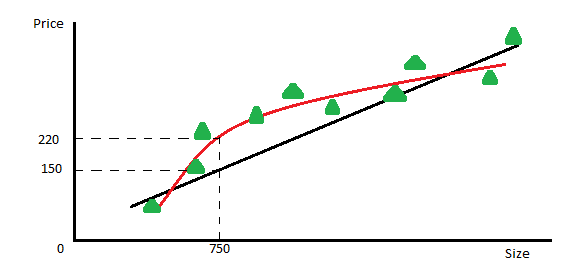
\includegraphics[width=5in,height=3.5in,keepaspectratio=true]{SoDoGiaNha.png}
	\caption{Dự đoán giá nhà}
\end{figure}\\
Bạn của bạn muốn thuê một căn phòng với diện tích là $750 feet^2$ và người đó
muốn biết giá trị khoảng bao nhiêu. Vậy các thuật toán của Machine Learning sẽ
giúp ta như thế nào?\\\\
Một điều mà có lẽ thuật toán có thể làm là đặt ra một
đường thẳng thông qua dữ liệu, dựa trên đó, có vẻ như giá ngôi nhà có thể là
150.000 \$.\\\\
Nhưng đó không phải là cách duy nhất mà thuật toán có thể xây dựng. Một cách tốt
hơn, thay vì một đường thẳng chúng ta có thể sử dụng một hàm quadratic hoặc một
đa thức bậc hai cho dữ liệu. Khi đó hàm sẽ được biểu diễn dưới dạng một đường
cong tương đối gần với dữ liệu được cho. Lúc này giá trị của ngôi nhà là 200.000
\$.\\\\
Vậy, quyết định như thế nào để chọn một trong hai phép phân tích trên?\\\\
Và đó là một ví dụ về Supervised Learning. Trong một số giới hạn nào đó,
Supervised Learing có thể chỉ ra thuật toán mà chúng ta sử dụng là một thuật
toán đúng.
\begin{itemize}
  \item Thuật ngữ Regression (Hồi quy): dự đoán giá trị tiếp theo, hoặc dự đoán
  thuộc tính của giá trị.\\\\
  Một số ví dụ khác về Supervised Learning: Ta đi dự đoán bệnh ung thư vú là ác
  tính hay lành tính từ thông tin một hồ sơ y tế.\\
  \begin{figure}[h!]
  	\centering
	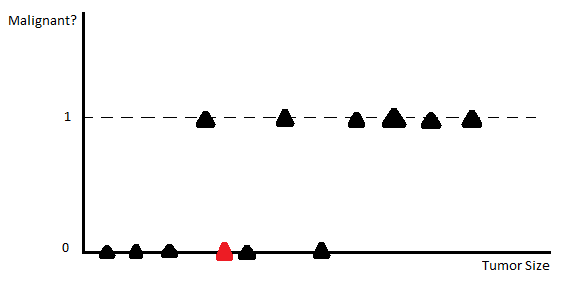
\includegraphics[width=5in,height=3.5in,keepaspectratio=true]{HoiQuy.png}
	\caption{Dự đoán ung thư}
\end{figure}\\
  Giả sử chúng ta có một người bạn, người bạn ấy có một khối u với kích thước
  tại vị trí đánh dấu (vị trí màu đỏ). Câu hỏi của Machine Learning là có thể
  ước lượng xác suất là bao nhiêu? Cơ hội để nó là khối u lành tính là bao
  nhiêu?  \\\\\\
  \item Thuật ngữ Classification: Sự phân loại. Ta đi làm rõ thuật ngữ này bằng
  ví dụ sau.\\\\
   Giả sử ta đơn giản hóa sơ đồ trên bằng sơ đồ sau:
   \begin{figure}[h!]
  	\centering
	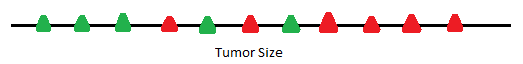
\includegraphics[width=6in,height=3.5in,keepaspectratio=true]{PhanLoai1.png}
	\caption{Biễn diễn ung thư theo kích thước khối u}
\end{figure}\\
	Trong đó:\\
	\tab Màu xanh là lành tính\\
	\tab Màu đỏ là ác tính\\\\
	Bây giờ, không chỉ còn biết về kích thước khối u mà ta còn biết về độ tuổi
	người bệnh. Ta hình thành sơ đồ bên dưới:\\
	 \begin{figure}[h!]
  	\centering
	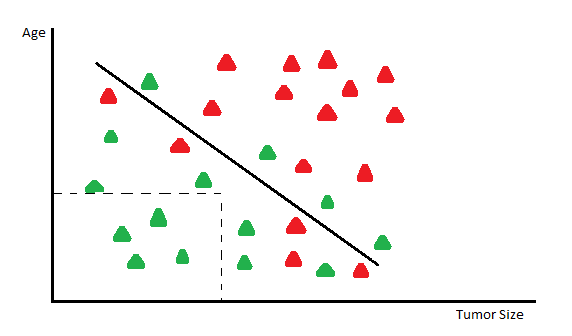
\includegraphics[width=5in,height=3.5in,keepaspectratio=true]{PhanLoai2.png}
	\caption{Biểu diễn ung thư theo kích thước khối u và lức tuổi}
\end{figure}\\
Ta có thể dựa vào độ tuổi của người bạn để cho ra kết quả dự đoán. Đó chính là
Classification.\\\\
Một vấn đề khác, ở các ví dụ trên ta chỉ dựa vào vài yếu tố, thuộc tính nhưng
Machine Learning lại khác, số lượng đầu vào các thuộc tính là rất nhiều. Vậy làm
thế nào để lưu khi bộ nhớ máy tính là giới hạn? Ta đi đến với một thuật toán gọi
là Support Vector Machine, và điều này sẽ được làm rõ ở các phần sau.
\end{itemize}
\subsubsection{Unsupervised Learning}
Trong phần trước, Supervised Learning được sỡ hữu một tập dữ liệu mà mỗi giá trị
đều được gắn và phân chia nhãn.\\
\begin{figure}[h!]
  	\centering
	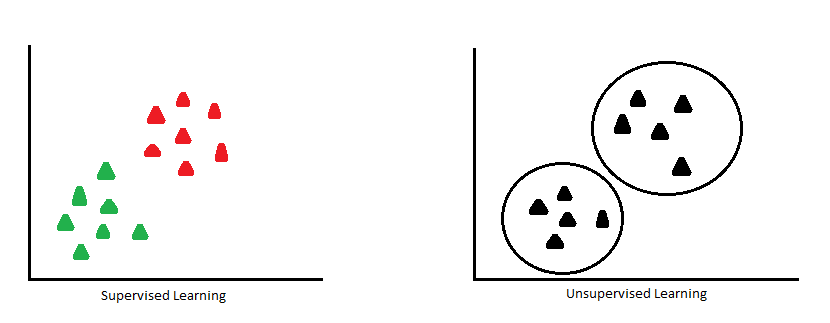
\includegraphics[width=5in,height=3.5in,keepaspectratio=true]{KhongGiamSat.png}
	\caption{Phân biệt supervised và unsupervised}
\end{figure}\\
Unsupervised Learning được sỡ hữu một tập dữ liệu khác hơn, tất cả đều cùng nhãn
hay khác hơn là có thể không có nhãn. Câu hỏi đặt ra của bài toán này là làm sao
tìm được cấu trúc của dữ liệu này?\\\\
Với dữ liệu trên, Unsupervised Learning
sẽ quyết định dữ liệu tồn tại trong hai nhóm, và đó gọi là thuật toán gom cụm -
Clustering Algorithm.
\section{Các thuật toán thu giảm số chiều}
\subsection{Principal Component Analysis - PCA}
Trước khi bắt đầu vào thuật toán, chúng ta sẽ đi tìm hiểu sơ qua về ý tưởng ban
đầu của thuật toán này. Với mục đích ban đầu là loại bỏ đi các chiều hay thuộc
tính không cần thiết của không gian ma trận dữ liệu đầu vào, ta sẽ đi xác định
những thuộc tính nào có tính quan trọng thấp để loại bỏ. Trong thuật toán này,
tính quan trọng của một thuộc tính được đo bằng khả năng phân loại của chúng, để
rõ ràng hơn ta đi quan sát hình ảnh bên dưới.\\\\ 
(Hình ảnh được trích từ
bộ slide môn học Machine Learning – GS. Cao Hoàng Trụ - Đại học Bách Khoa
TP.HCM)\\
\begin{figure}[h!]
  	\centering
	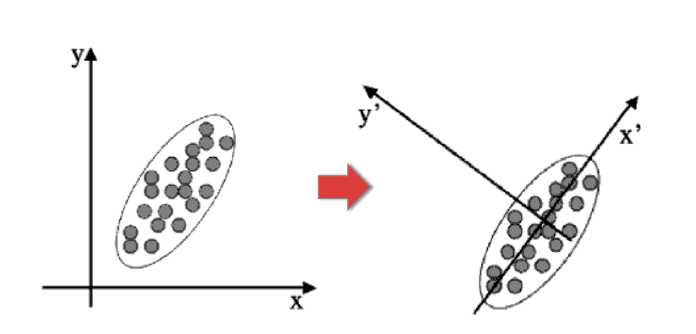
\includegraphics[width=5in,height=3.5in,keepaspectratio=true]{PCA.png}
	\caption{PCA}
\end{figure}\\
Hãy thử tưởng tượng, hình ảnh bên tay trái là bộ dữ liệu đầu vào ban đầu và gồm
hai thuộc tính là x và y. Ta đi thu giảm số chiều, nghĩa là bây giờ ta muốn chỉ
cần dùng một thuộc tính để đại diện cho tập dữ liệu. Có hai lựa chọn x’ và y’ –
hình ảnh bên tay phải.\\\\ 
Theo như một cách nghĩ trực quan nhất thì ta
thấy việc chiếu theo chiều y’ sẽ khiến cho tập dữ liệu bị gom lại rất gần nhau
và nó được xem là không có tính phân loại cao. Xem xét việc chiếu theo chiều x’,
ta dễ dàng nhận thấy tập dữ liệu được kéo dãn ra so với y’, do đó, chiều x’ được
xem là chiều giúp cho tập dữ liệu dù bị loại bớt thuộc tính nhưng vẫn giữ được
tính phân loại bên trong nó.\\\\ 
 Từ ý tưởng trên, chúng ta sẽ đi xây dựng
mô hình toán học. Đơn giản, độ đo gom cụm hay kéo dãn của tập dữ liệu khi chiếu
lên một chiều vector sẽ được biễu diễn bằng khái niệm phương sai của tập dữ liệu
trên chiều vector đó.\\\\
Gọi tập dữ liệu là tập hợp n vector $\{x_i\}_{i=1,\dots,n}$. Ta có:\\
Vector trung bình:
\[ m = \frac{1}{n} \sum_{i=1}^{n} x_i \]
Phương sai của dữ liệu chiếu theo chiều u:
\[ \frac{1}{n}\sum_{i=1}^{n} (u^T.x_i - u^T.m)^2 = u^T.S.u \]
Với:
\[ S= \frac{1}{n}\sum_{i=1}^n (x_i-m).(x_i-m)^T \]
Và S là ma trận đối xứng.\\\\
Bài toán là cần tìm một chiều vector dùng để chiếu xuống có tính phân loại cao
đồng nghĩa với việc phương sai của tập dữ liệu trên chiều vector đó cực đại. Vậy
nhiệm vụ của chúng ta sẽ đi tìm u để cực đại phương sai:\\\\
Bài toán cực đại:
\[ \frac{1}{n}\sum_{i=1}^{n} (u^T.x_i - u^T.m)^2 = u^T.S.u \]
Không làm thay đổi tính chất bài toán, ta chọn u là vector đơn vị, nghĩa là:
\[ u^Tu= ||u||^2= 1 \]
Với bài toán cực đại có điều kiện, ta sẽ sử dụng Lagrangian.\\\\
Cực đại hàm Lagrangian:
\[ L(u,\lambda) = u^T.S.u + \lambda(1-u^Tu) \]
Đạo hàm theo $L(u,\lambda)$ theo u:
\[ \frac{\partial L}{\partial u} = \nabla_u u^T.S.u + \nabla_u \lambda(1-u^Tu) =
\nabla_uu^T.S.u -\lambda \nabla_uu^Tu \] 
Đặt:
\begin{align}
& \nabla_uu^T.S.u\\
& \lambda \nabla_uu^Tu
\end{align}
Xét (3.1):
\[ (3.1) = \nabla_uu^T.S.u = 2u^TS \]
Xét (3.2):
Giả sử
\begin{align}
x = \begin{bmatrix} x_1 \\ \vdots \\ x_n \end{bmatrix} \Rightarrow
x^T.x & = x_1^2 + \dots + x_n^2 = X
\nabla_xx^Tx \notag\\
& = \begin{bmatrix} \frac{\partial X}{\partial x_1} & \dots &
\frac{\partial X}{\partial x_n} \end{bmatrix} = \begin{bmatrix}
2x_1 & \dots & 2x_n \end{bmatrix} = 2x^T\notag
\end{align}
Suy ra:
\[ (3.2) = \lambda \nabla_uu^Tu = 2\lambda u^T \]
Từ biến đổi (3.1) và (3.2):
\[ \frac{\partial L}{\partial u} = 2u^TS - 2\lambda u^T \]
Đặt vế phải biểu thức bằng 0 ta được:
\begin{align}
& 2u^TS - 2\lambda u^T = 0\notag\\
&\Leftrightarrow 2u^TS = 2\lambda u^T\notag\\
&\Leftrightarrow (u^TS)^T = (\lambda u^T)^T\notag\\
&\Leftrightarrow Su = \lambda u\notag
\end{align}
Tại đây ta có thể nhận ra, phương sai của tập dữ liệu khi chiếu lên vector u cực
đại khi và chỉ khi u là eigenvector của S và $\lambda$ là eigenvalue của S. Từ
đó ta suy ra:
\[ S= 
\begin{bmatrix}
u_1 & u_2 & \dots & u_n
\end{bmatrix} 
\begin{bmatrix}
\lambda_1 & 0 & \dots & 0 \\
0 & \lambda_2 & \dots & 0 \\
\vdots & \vdots & \ddots & \vdots \\
0 & 0 & \dots & \lambda_n 
\end{bmatrix}
\begin{bmatrix}
u_1 & u_2 & \dots & u_n
\end{bmatrix} ^{-1}
\]
Với $u_1,u_2,\dots,u_n$ là các eigenvector của S và
$\lambda_1,\lambda_2,\dots,\lambda_n$ là các eigenvalue của S tương ứng với
eigenvector.\\\\ 
Ta thu giảm không gian vector bây giờ tương ứng với việc ta loại bỏ đi những
vector u mà ta cho là không cần thiết. Công việc loại bỏ này được thực hiện bằng
cách chọn một giá trị $\lambda$ làm mốc, sau đó ta loại bỏ những eigenvalue của
S có giá trị nhỏ hơn $\lambda$ và cũng loại bỏ luôn những eigenvector tương
ứng.\\\\ 
Vậy, sau khi loại bỏ xong, ta chiếu tập dữ liệu ban đầu lên không gian vector
$u_1,u_2,\dots,u_m$ mới với m < n. Và lúc này ta được một tập dữ liệu, giữ lại
được tương đối thông tin của tập dữ liệu ban đầu nhưng đã được thu giảm số chiều vector.
\subsection{Singular Value Decomposition - SVD}
Singular Value Decomposition (SVD) có thể được xem xét từ ba điểm tương thích
lẫn nhau của cách nhìn nhận. Một mặt, chúng ta có thể xem nó như là một phương
pháp để chuyển biến tương quan vào một tập hợp của biến không tương quan mà
trình bày tốt hơn các mối quan hệ khác nhau của dữ liệu gốc. Đồng thời, SVD là
một phương pháp để xác định và sắp xếp thứ tự chiều dọc theo đó điểm dữ liệu
trình bày tối đa phương sai. Điều này gắn với cách thứ ba của cách nhìn SVD, đó
là một khi chúng ta đã xác định được nơi mà tối đa phương sai, nó có thể tìm
thấy xấp xỉ tốt nhất của các điểm dữ liệu ban đầu sử dụng ít chiều hơn. Do đó,
có thể SVD được xem như một phương pháp để giảm số chiều của dữ liệu.\\\\
Hãy xem xét các điểm dữ liệu 2 chiều trong hình 1. Đường hồi quy chạy qua chúng
cho thấy xấp xỉ tốt nhất của dữ liệu gốc với một đối tượng 1 chiều (một đường
thẳng). Nó là xấp xỉ tốt nhất theo nghĩa rằng nó là đường thẳng tối thiểu khoảng
cách giữa mỗi điểm ban đầu và đường thẳng. Nếu chúng ta vẽ một đường thẳng vuông
góc từ mỗi điểm đến đường hồi quy, và lấy giao điểm của những đường thẳng đó như
xấp xỉ của các điểm dữ liệu ban đầu, chúng ta sẽ có một đại diện của dữ liệu gốc
đã được thu giảm số chiều mà thu thập càng nhiều các phương sai gốc càng tốt.
Lưu ý rằng có một đường hồi quy thứ hai, vuông góc với dữ liệu ban đầu, thể hiện
trong hình 2. Đường thẳng này thu thập càng nhiều các phương sai nhất có thể
theo chiều thứ hai của tập dữ liệu gốc. Nó thực hiện xấp xỉ dữ liệu ban đầu kém
hơn so với hình 1, vì nó tương ứng với trình bày dữ liệu một chiều ít phương sai
hơn so với ban đầu. Có thể sử dụng các đường hồi quy để tạo ra một tập hợp các
điểm dữ liệu không tương quan sẽ hiển thị các tập con trong dữ liệu gốc không
nhất thiết phải hiển thị ở cái nhìn đầu tiên.\\
\begin{figure}[h!]
	\centering 
	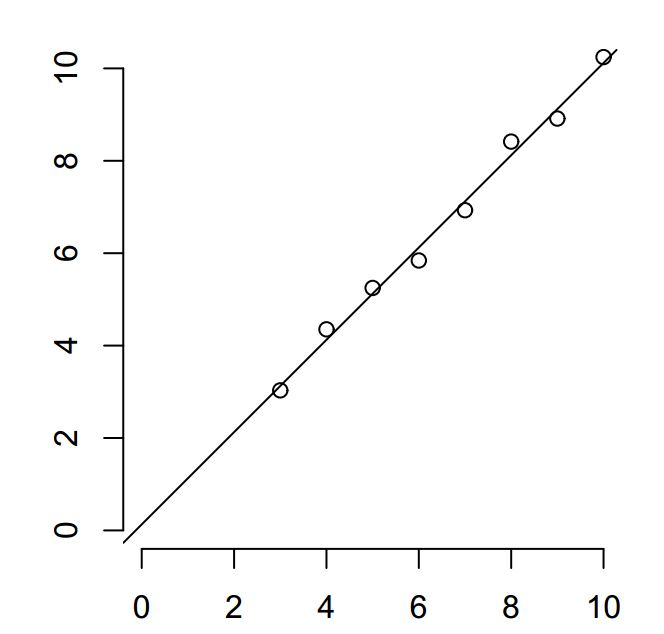
\includegraphics[width=4in,height=2in,keepaspectratio=true]{SVD1.png}
	\caption{Đường hồi quy phù hợp nhất giảm dữ liệu từ hai chiều thành một}
\end{figure}\\
Những ý tưởng cơ bản đằng sau SVD là: Ta lấy một bộ dữ liệu biến thiên rất cao
và có số chiều lớn, thu giảm nó đến một không gian chiều thấp hơn cho thấy nhiều
phần cấu trúc của các dữ liệu ban đầu rõ ràng hơn và thứ tự của nó từ những
phương sai nhiều nhất đến ít nhất. Điều làm cho SVD thiết thực trong các ứng
dụng xử lí ngôn ngữ tự nhiên chỉ đơn giản là có thể bỏ qua sự thay đổi dưới một
ngưỡng cụ thể để giảm lượng lớn dữ liệu, nhưng vẫn đảm bảo rằng mối quan hệ
chính của tỉ lệ được bảo đảm.\\
\begin{figure}[h!]
	\centering 
	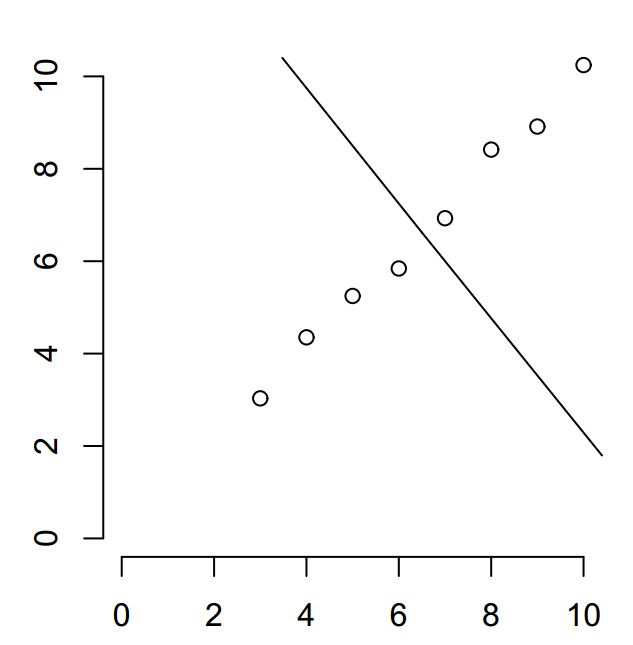
\includegraphics[width=4in,height=2in,keepaspectratio=true]{SVD2.png}
	\caption{Đường hồi quy theo chiều hướng thứ hai thu thập ít sự thay đổi phương
	sai trong dữ liệu gốc}
\end{figure}

\subsubsection{Thuật toán}
SVD được dựa trên một định lý từ đại số tuyến tính rằng một ma trận chữ nhật A
có thể được chia thành các tích của ba ma trận theo thứ tự - một ma trận trực
giao U, một ma trận đường chéo S, và chuyển vị của một ma trận trực giao V.
Định lý thường được trình bày theo công thức
\[ A_{mn} = U_{mm}S_{mn}V_{nn}^T \]
mà $U^TU = I, V^TV = I$, trong đó các cột của ma trận U là eigenvectors trực
giao của tích hai ma trận A và $A^T$, các cột của ma trận V là eigenvectors
trực giao của tích hai ma trận $A^T$ và A, và S là một ma trận đường chéo chứa
các căn bậc hai của các eigenvalue của ma trận U hoặc ma trận V theo thứ tự giảm dần.\\\\
Các bước để hiện thực SVD\\
\textbf{Bước 1:} Từ ma trận thuộc tính A ban đầu ta tính ma trận trực giao U
\begin{itemize}
  \item Tính tích hai ma trận theo thứ tự là A  và $A^T$.
  \item Tìm eigenvalues và eigenvectors tương ứng của tích hai ma trận A và
  $A^T$.
  \item Các eigenvectors trở thành vector cột trong một ma trận được sắp xếp
  theo kích thước của eigenvalue tương ứng. Nói cách khác, các eigenvectors của
  eigenvalue lớn nhất là cột một, các eigenvectors của eigenvalue lớn thứ hai
  theo là cột hai,\ldots và như vậy cho đến khi có các eigenvectors của
  eigenvalue nhỏ nhất như cột cuối cùng của ma trận.
  \item Cuối cùng, chúng ta phải chuyển đổi ma trận này thành một ma trận trực
  giao bằng cách áp dụng quá trình trực chuẩn hóa Gram-Smith với vector cột.
\end{itemize}
\textbf{Bước 2:} Từ ma trận thuộc tính A ban đầu ta tính ma trận trực giao V
giống như tính toán ma trận trực giao U tuy nhiên ta sẽ tính bằng tích hai ma
trận theo thứ tự là $A^T$ và A (của U là A và $A^T$).\\
\textbf{Bước 3:} Đối với ma trận S ta lấy căn bậc hai của các eigenvalues khác
không và đặt trong đường chéo của ma trận S, eigenvalues lớn nhất là $s_{11}$,
eigenvalues tiếp theo là $s_{22}$ và cứ thế cho đến giá trị eigenvalues nhỏ nhất
là $s_{mm}$. Các eigenvalues khác không của ma trận U và V là luôn luôn giống
nhau, vì vậy đó là lý do tại sao nó không quan trọng trong việc chúng ta lấy
eigenvalues của ma trận nào. Tất cả các giá trị còn lại của ma trận S là giá trị
không.\\
\textbf{Bước 4:} Thu giảm số chiều của ba ma trận U, S và V.
\subsubsection{Thu giảm số chiều của ma trận thuộc tính}
S chứa căn bậc hai của các giá trị theo thứ tự từ lớn nhất đến nhỏ nhất của nó
theo đường chéo. Những giá trị này cho thấy phương sai của các thành phần độc
lập tuyến tính dọc theo mỗi chiều. Ta thực hiện loại bỏ các giá trị nhỏ theo
đường chéo của ma trận bằng cách loại bỏ toàn bộ hàng chứa giá trị đó. Để cho
phép nhân ma trận, chúng ta phải loại bỏ sự tương ứng vector hàng của U và
vector cột tương ứng của $V^T$ để được kết quả là xấp xỉ của ma trận A ban đầu.\\\\
Đây là một ví dụ cụ thể
\[ A =
\begin{bmatrix}
2 & 0 & 8 & 6 & 0 \\
1 & 6 & 0 & 1 & 7 \\
5 & 0 & 7 & 4 & 0 \\
7 & 0 & 8 & 5 & 0 \\
7 & 0 & 8 & 5 & 0
\end{bmatrix} \]
Ta đưa ma trận A thành $USV^T$
\[ U =
\begin{bmatrix}
-0.54 & 0.07 & 0.82 & -0.11 & 0.12 \\
-0.10 & -0.59 & -0.11 & -0.79 & -0.06 \\
-0.53 & 0.06 & -0.21 & 0.12 & -0.81 \\
-0.53 & 0.06 & -0.21 & 0.12 & -0.81 \\
-0.06 & -0.80 & 0.09 & 0.59 & 0.04
\end{bmatrix} \]
\[ V^T =
\begin{bmatrix}
-0.46 & 0.02 & -0.87 & 0 & 0.17 \\
-0.07 & -0.76 & 0.06 & 0.60 & 0.23 \\
-0.07 & -0.76 & 0.06 & 0.60 & 0.23 \\
-0.48 & 0.03 & 0.40 & -0.33 & 0.70 \\
-0.07 & -0.64 & -0.04 & -0.69 & -0.32
\end{bmatrix} \]
Eigenvalue trong quá trình tính toán là $\lambda = 321.07, \lambda = 230.17, \lambda =
12.70, \lambda = 3.94, \lambda = 0.12$.
Ta sẽ có ma trận S là ma trận có đường chéo là các eigenvalue theo thứ tự từ lớn
đến nhỏ. Để minh họa ảnh hưởng của giảm chiều trên tập dữ liệu này, chúng ta sẽ hạn chế S với ba giá trị số ít đầu tiên để có được
\[\begin{bmatrix}
17.92 & 0 & 0 \\
0 & 15.17 & 0 \\
0 & 0 & 3.56 
\end{bmatrix} \]
Ta thu giảm tương ứng số cột của ma trận U và số hàng của ma trận $V^T$ xuống
bằng số hàng của ma trận S mà tính phép nhân ma trận ta có được ma trận
$\widehat{A}$ xấp xỉ ma trận A bằng
\[ \widehat{A} = 
\begin{bmatrix}
-0.54 & 0.07 & 0.82 \\
-0.10 & -0.59 & -0.11\\
-0.53 & 0.06 & -0.21\\
-0.53 & 0.06 & -0.21\\
-0.06 & -0.80 & 0.09
\end{bmatrix}
\begin{bmatrix}
17.92 & 0 & 0 \\
0 & 15.17 & 0 \\
0 & 0 & 3.56 
\end{bmatrix}
\begin{bmatrix}
-0.46 & 0.02 & -0.87 & 0 & 0.17 \\
-0.07 & -0.76 & 0.06 & 0.60 & 0.23 \\
-0.74 & 0.10 & 0.28 & 0.22 & -0.56
\end{bmatrix} 
\]
\[ = 
\begin{bmatrix}
2.29 & -0.66 & 9.33 & 1.25 & -3.09 \\
1.77 & 6.76 & 0.90 & -5.50 & -2.13 \\
4.86 & -0.96 & 8.01 & 0.38 & -0.97 \\
6.62 & -1.23 & 9.58 & 0.24 & -0.71 \\
1.14 & 9.19 & 0.33 & -7.19 & -3.13
\end{bmatrix} 
\]
Tuy nhiên, trong thực tế, mục đích không phải là để tái tạo lại các ma trận ban
đầu, nhưng sử dụng để giảm số chiều đại diện để xác định thuộc tính và các dữ
liệu đầu vào tương tự. Những dữ liệu đầu vào (observation) được đại diện bởi các
vector hàng trong ma trận V, và dữ liệu đầu vào tương tự thu được bằng cách so
sánh các hàng trong tích ma trận V.S (lưu ý rằng các dữ liệu đầu vào được biểu
diễn như là vector hàng bởi vì chúng ta đang làm việc với V, không phải $V^T$).
thuộc tính được biểu diễn bằng vector hàng trong U, và thuộc tính tương tự có
thể thu được bằng cách tính tương tự hàng ở tích ma trận U.S. Thay vì xử lí thuộc tính
của dữ liệu trên một ma trận có 5 cột như ma trận A ban đầu, giờ đây ta chỉ cần
xử lí thuộc tính của dữ liệu trên một ma trận có giá trị xấp xỉ ma trận A ban
đầu nhưng chỉ có 3 cột.\\\\     
Chúng ta biết rằng các vector chứa phần tử theo thứ tự từ lớn nhất đến ít nhất
của phương sai trong dữ liệu gốc. Bằng cách xóa các phần tử đại diện cho số
chiều mà không thể hiện phương sai có nghĩa, chúng ta có thể loại bỏ sự nhiễu dữ
liệu hiệu quả trong thuộc tính. Bây giờ vector thuộc tính là ngắn hơn, và chỉ
chứa các phần tử giải thích cho sự tương quan đáng kể nhất trong số các thuộc
trong tập dữ liệu ban đầu.
\section{Tổng quan về hệ thống phát hiện xâm nhập trên host - HIDS}
\subsection{Khái niệm về hệ thống phát hiện xâm nhập - IDS}
   IDS là viết tắt của từ Intrusion detection system, có nghĩa là hệ thống phát
  hiện xâm nhập. Hệ thống phát hiện xâm nhập là hệ thống được phát triển nhằm
  mục đích bảo vệ máy tính khỏi sự xâm nhập trái phép hoặc sự sử dụng trái với
  quy định.\\\\ 
   Hệ thống này có thể là phần mềm cài đặt trên máy tính, thiết bị mạng, hoặc là
   thiết bị phần cứng đặt trên đường truyền để giám sát đường truyền
   mạng.\\\\ 
Hệ thống phát hiện xâm nhập (IDS) chỉ thực hiện công việc giám sát các hoạt động
và đưa ra cảnh báo cho admin. Admin sẽ dựa vào cảnh báo từ hệ thống IDS để xác
định hành động kế tiếp.\\\\ 
 Hệ thống IDS không có chức năng tự động ngắt bỏ hay ngăn chặn hành động trái
 phép, thay vào đó là hệ thống IPS (Intrusion prevention system), hệ thống ngăn
 chặn xâm nhập sẽ thực hiện công việc này.\\\\ 
 Hệ thống IDS có 2 loại: HIDS và NIDS.
\subsection{Hệ thống phát hiện xâm nhập trên mạng - NIDS}
  NIDS là viết tắt của từ Network-base Intrusion Detection System, có nghĩa là
  hệ thống phát hiện xâm nhập trên network. Hệ thống này thường được cài đặt
  trên các thiết bị mạng là gateway của mạng nội bộ, hoặc là thiết bị phần cứng
  lắp đặt trên đường truyền giữa mạng ngoài và mạng nội bộ.\\\\ 
   Chức năng chính của hệ thống này là giám sát hoạt động mạng của toàn bộ các
   thiết bị nằm trong phần mạng nội bộ với mạng ngoài, mục đích là để bảo vệ
   toàn bộ mạng nội bộ khỏi các cuộc tấn công mạng và các virus.\\\\ 
    Dữ liệu kiểm tra của NIDS là các gói tin truyền trên mạng, NIDS thực hiện
    kiểm tra các giao thức, header gói tin, nội dung gói tin để tìm ra các dấu
    hiệu khả nghi. \\\\ 
    Nhưng việc kiểm tra các gói tin trên đường truyền
    mạng có các bất cập sau:
    \begin{itemize}
      \item Dữ liệu truyền nhận có thể đã bị mã hóa do các giao thức bảo mật,
      như vậy việc rút trích thông tin để phát hiện xâm nhập là vô cùng khó.
      \item Gói tin trên đường truyền có thể bị phân mảnh, nội dung gói tin
      không còn hoàn chỉnh, như vậy việc phân tích gói tin cũng không khả thi.
    \end{itemize}
    \begin{figure}[h!]
	\centering 
	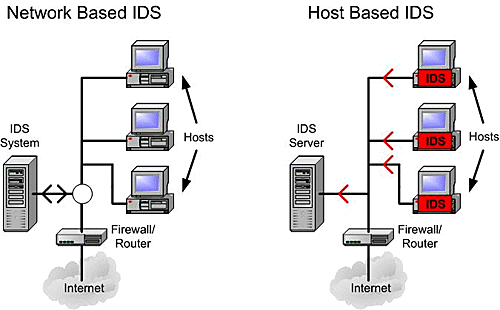
\includegraphics[width=6in,height=3in,keepaspectratio=true]{HIDS_NIDS.png}
	\caption{So sánh giữa NIDS và HIDS}
\end{figure}
\subsection{Hệ thống phát hiện xâm nhập trên host - HIDS}
  HIDS là viết tắt của từ Host-base Intrusion Detection System, có nghĩa là hệ
  thống phát hiện xâm nhập trên host. Hệ thống này được cài đặt trên từng máy
  tính.\\\\  
  Chức năng chính của hệ thống này là giám sát hoạt động của 1 máy tính riêng
  lẻ, kể cả các dữ liệu mạng cũng như các hoạt động trong bản thân máy tính,
  kiểm tra hoạt động của máy tính để phát hiện sự xâm nhập và cảnh báo cho
  admin.\\\\ 
  Dữ liệu kiểm tra của HIDS là các gói tin hoàn chỉnh, các lời gọi hàm (system
  call), các file log trong máy tính. HIDS thực hiển kiểm tra các header, địa
  chỉ IP gói tin, cũng như nội dung gói tin, ngoài ra còn có giám sát việc thực
  thi chương trình thông qua lời gọi hàm và các file log.
\subsection{Hình thức phát hiện xâm nhập}
  Cả 2 loại IDS đều có 2 hình thức phát hiện xâm nhập sau:
  \begin{enumerate}
    \item Signature base: Kiểu phát hiện xâm nhập dựa trên đặc điểm nhận dạng
    của đối tượng. Trong hình thức này, tất cả mọi kiểu xâm nhập đều đã được đưa
    ra các đặc điểm nhận dạng và lưu vào trong cơ sở dữ liệu trong hệ thống. Hệ thống khi bắt được 1 sự kiện sẽ so sánh với tập dữ liệu nhận dạng này, nếu trùng với đặc điểm nhận dạng thì hệ thống sẽ báo ngay.
    \begin{itemize}
      \item Ưu điểm: Có tốc độ nhanh, do chỉ việc so sánh trùng với dữ liệu.
      \item Nhược điểm: Đối với kiểu xâm nhập chưa được nhận diện thì không phát
      hiện được, nên phải thường xuyên cập nhật các dấu hiệu nhận dạng của đối tượng xâm nhập.
    \end{itemize}
     
	\item Behavior base: Kiểu phát hiện xâm nhập dựa trên hành vi của chương
	trình. Trong hình thức này, các hoạt động của chương trình được lưu lại. Một
	khi có những hoạt động không bình thường trong chương trình, hệ thống sẽ kích
	hoạt cảnh báo. Các hoạt động bất thường có thể là sự tăng đột ngột số request
	tới server, công suất CPU bị đẩy lên tối đa tại 1 thời điểm.
	 \begin{itemize}
	   \item Ưu điểm: Có thể phát hiện ra những kiểu xâm nhập mà signature base không phát
	 hiện được.
	 \item Khuyết điểm: Cơ hội nhận diện sai thường sẽ cao hơn, do việc so sánh hành vi
	không thật sự chính xác.
	\end{itemize}
  \end{enumerate}
\subsection{Các chức năng chính trong HIDS}
  \begin{itemize}
    \item Kiểm tra tính toàn vẹn của file: Sử dụng các hàm mật mã như hàm hash
    để tạo ra chuỗi checksum cho file, sau đó theo thời gian định trước so sánh checksum của file với checksum cũ để kiểm tra tính toàn vẹn.
    \item Giám sát thanh ghi trên hệ điều hành Windows:
Hệ thống thanh ghi trên hệ điều hành Windows chứa các cấu hình về thiết bị phần cứng cũng như phần mềm của máy, mỗi lần có sự thay đổi trong hệ thống thanh ghi này đều được HIDS ghi lại để phát hiện những hành động trái quy định.
    \item Kiểm tra rootkit:
Rootkit là các chương trình được cài ẩn trong hệ thống mà người dùng không biết, rootkit được sử dụng để tạo ra các dịch vụ, chương trình chạy ngầm, nhầm mục đích là để cho Intruders có thể khống chế máy tình hoặc làm việc theo ý muốn.
Hệ thống HIDS có cơ chế kiểm tra việc cài đặt và thực thi cũng những chương trình này.
    \item Active response:
Active response là việc 1 chương trình thực thi sẽ kích hoạt thực thi của chương trình khác, cơ chế này giúp cho HIDS sau khi phát hiện xâm nhập có thể có những hành động kịp thời để bảo vệ máy tính.
  \end{itemize}